\documentclass[a0,final, portrait]{inriaposter}

\usepackage[utf8]{inputenc}
\usepackage[OT1]{fontenc}
\usepackage[english]{babel}
\usepackage{amsfonts, amsmath, amssymb, amsthm, dsfont, amsthm}
\usepackage{paralist}
\usepackage{wrapfig}

\usepackage{caption}
\usepackage{subcaption} 

\usepackage{graphics}
\usepackage{graphicx}

\usepackage{epstopdf}

\providecommand{\mtx}[1]{\mathbf{#1}}

\begin{document}

\sffamily

\postertitle%
{Interactive Learning from \\ Unlabeled Instructions}
{Jonathan Grizou \textsuperscript{1} \; and \; Iñaki Iturrate\textsuperscript{2} \; and \\ Luis Montesano\textsuperscript{3} \; and \; Pierre-Yves Oudeyer\textsuperscript{1} \; and \; Manuel Lopes\textsuperscript{1}}{\Large  \textsuperscript{1} Flowers Team,  INRIA / ENSTA ParisTech, France \; --- \; \textsuperscript{2} CNBI, EPFL, Switzerland \; --- \; \textsuperscript{3} I3A, University of Zaragoza, Spain}

\vfill
\Large
\begin{multicols}{2}

\blockabstract{
\textbf{Can a system learn a task from human instructions if it does not known how to interpret the human communicative signals?} 

In human-robot interaction, tutoring systems, and in human-computer interfaces such as brain-computer ones, the user should often go through a calibration procedure before interacting with the system. We address the problem of removing this calibration procedure. This has important practical application since the user can start controlling a device from scratch, without the need of an expert to define the meaning of signals or carrying out a calibration phase. 
}

\block{How it works}{

We exploits task constraints to build a distribution of possible tasks, and generate interpretation hypothesis of the EEG signals according to each hypothetic task. 


\begin{center}
	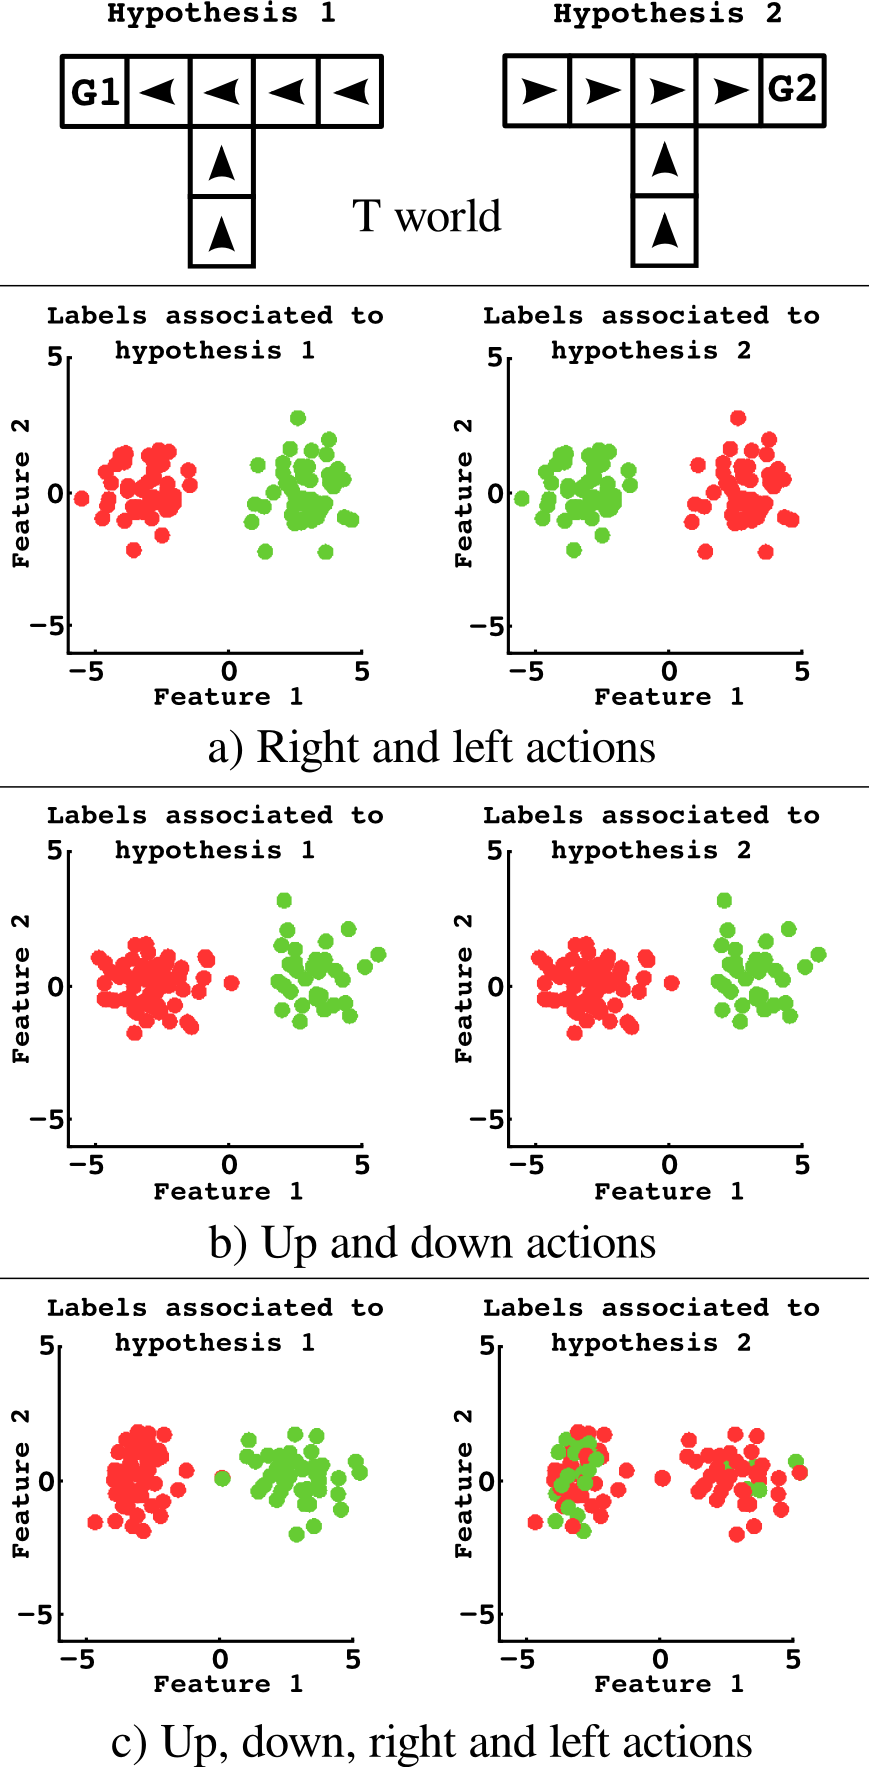
\includegraphics[width=0.7\columnwidth]{images/planning.png}
\end{center}

{\large A “T world” scenario and the interpretation hypothesis for different planning strategies. The agent knows it should reach either of the two edges of the T world (marked with the letter G). For each move the agent receives an unlabeled two dimensional teaching signal, corresponding to user’s assessments on the agent’s actions. The teacher’s goal is to have the agent reach G1. As the agent do not have access to this information, it interprets the signal according to each hypothesis (G1 and G2). a) shows the interpretation results if the agent only perform right and left actions in the top of the T world, b) shows the interpretation results when the agent only performs up and down actions in the trunk of the T, and c) shows the interpretation results for an agent performing all possible actions. Only the method c) allow to differentiate between hypothesis.}


% We select the hypothesis which best explains the history of interaction. Since the correct task will assign the correct labels to the signals, and the wrong task will assign some wrong labels, the expected classification rate is a good measure to identify the user's intended task. 

}



\block{Results}{

The user can start controlling a device from scratch, without the need of a calibration procedure.

\begin{center}
	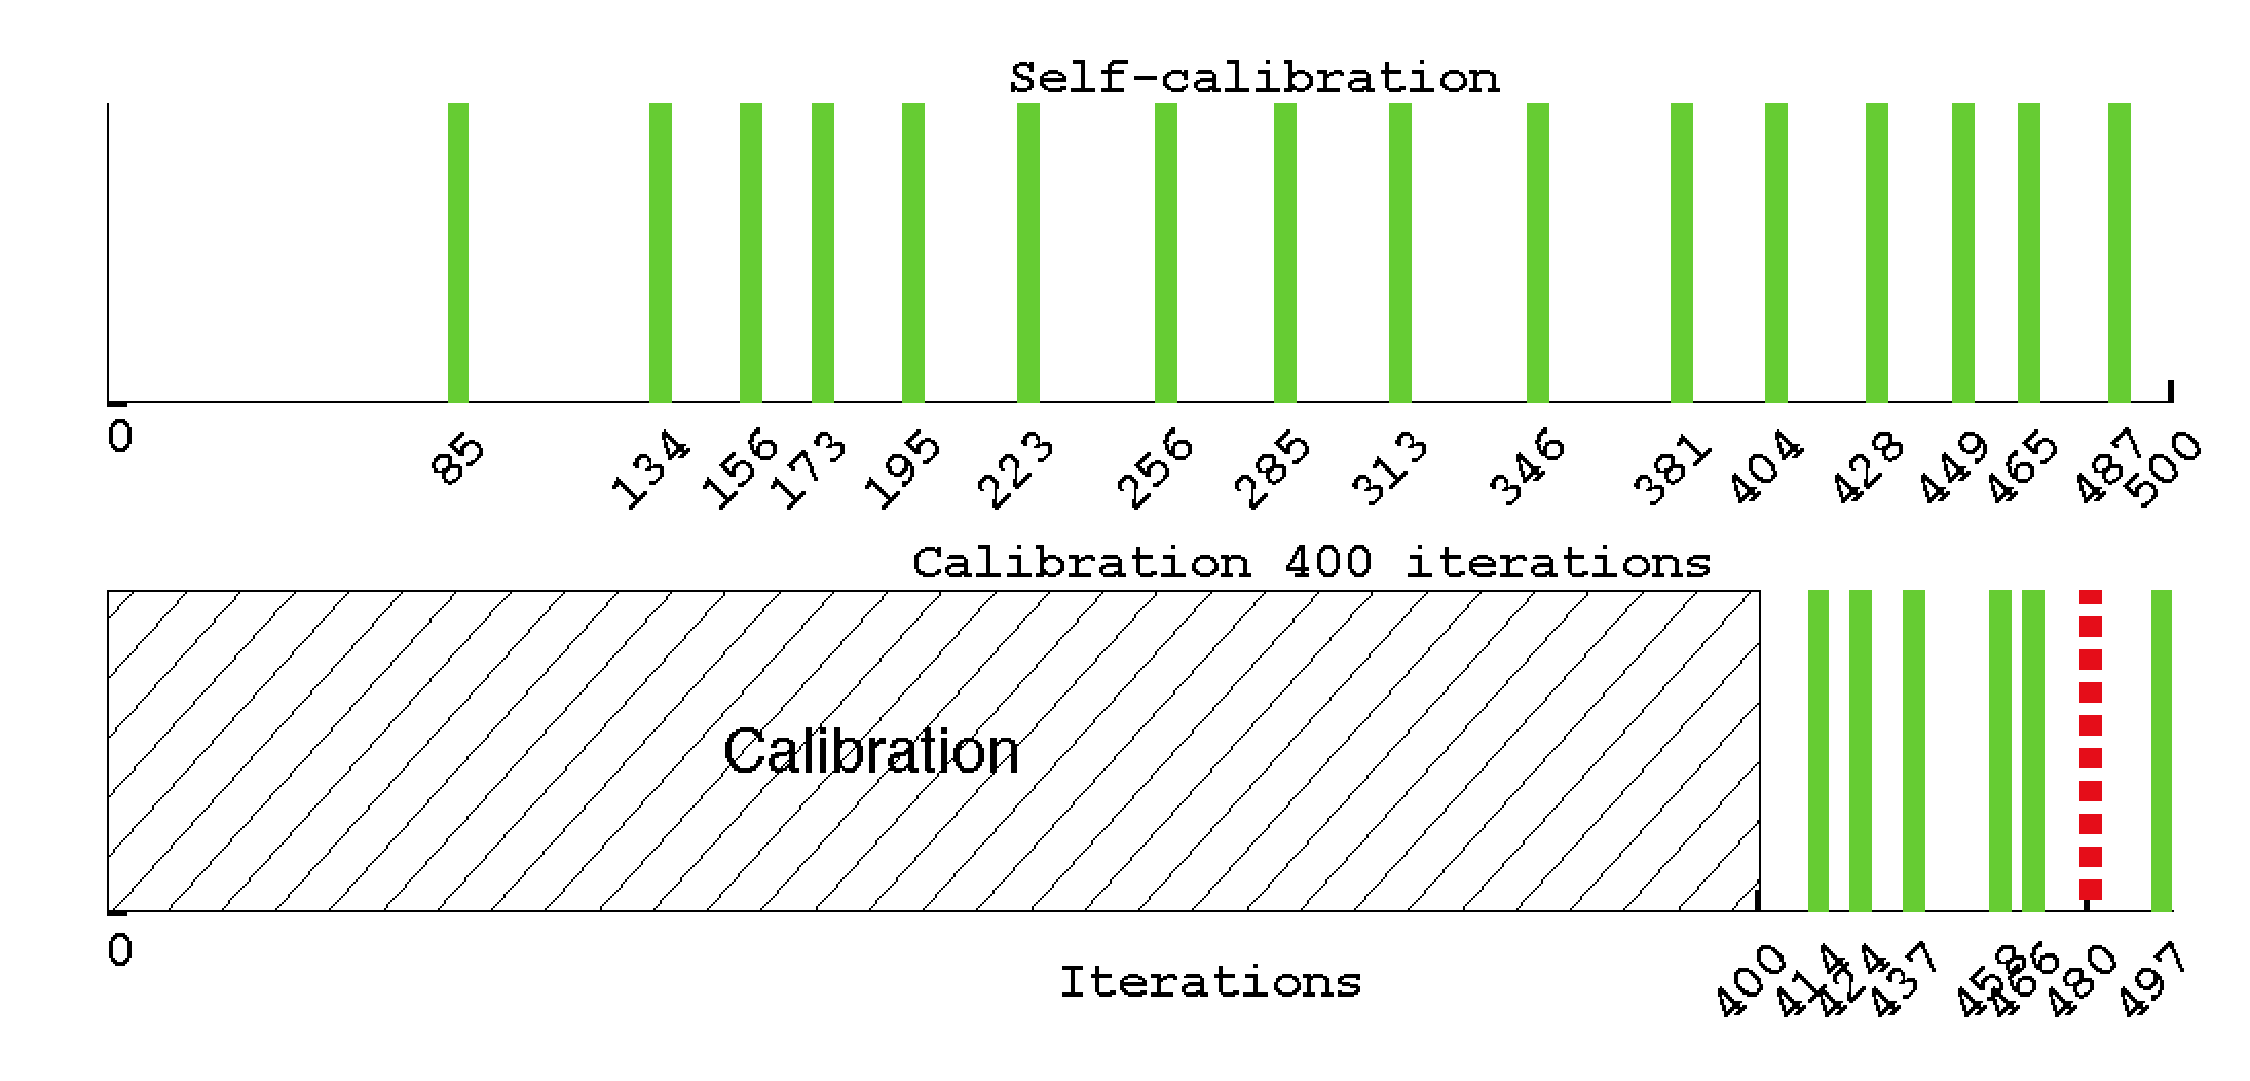
\includegraphics[width=0.8\columnwidth]{images/plot_the_aaai_sequence}
	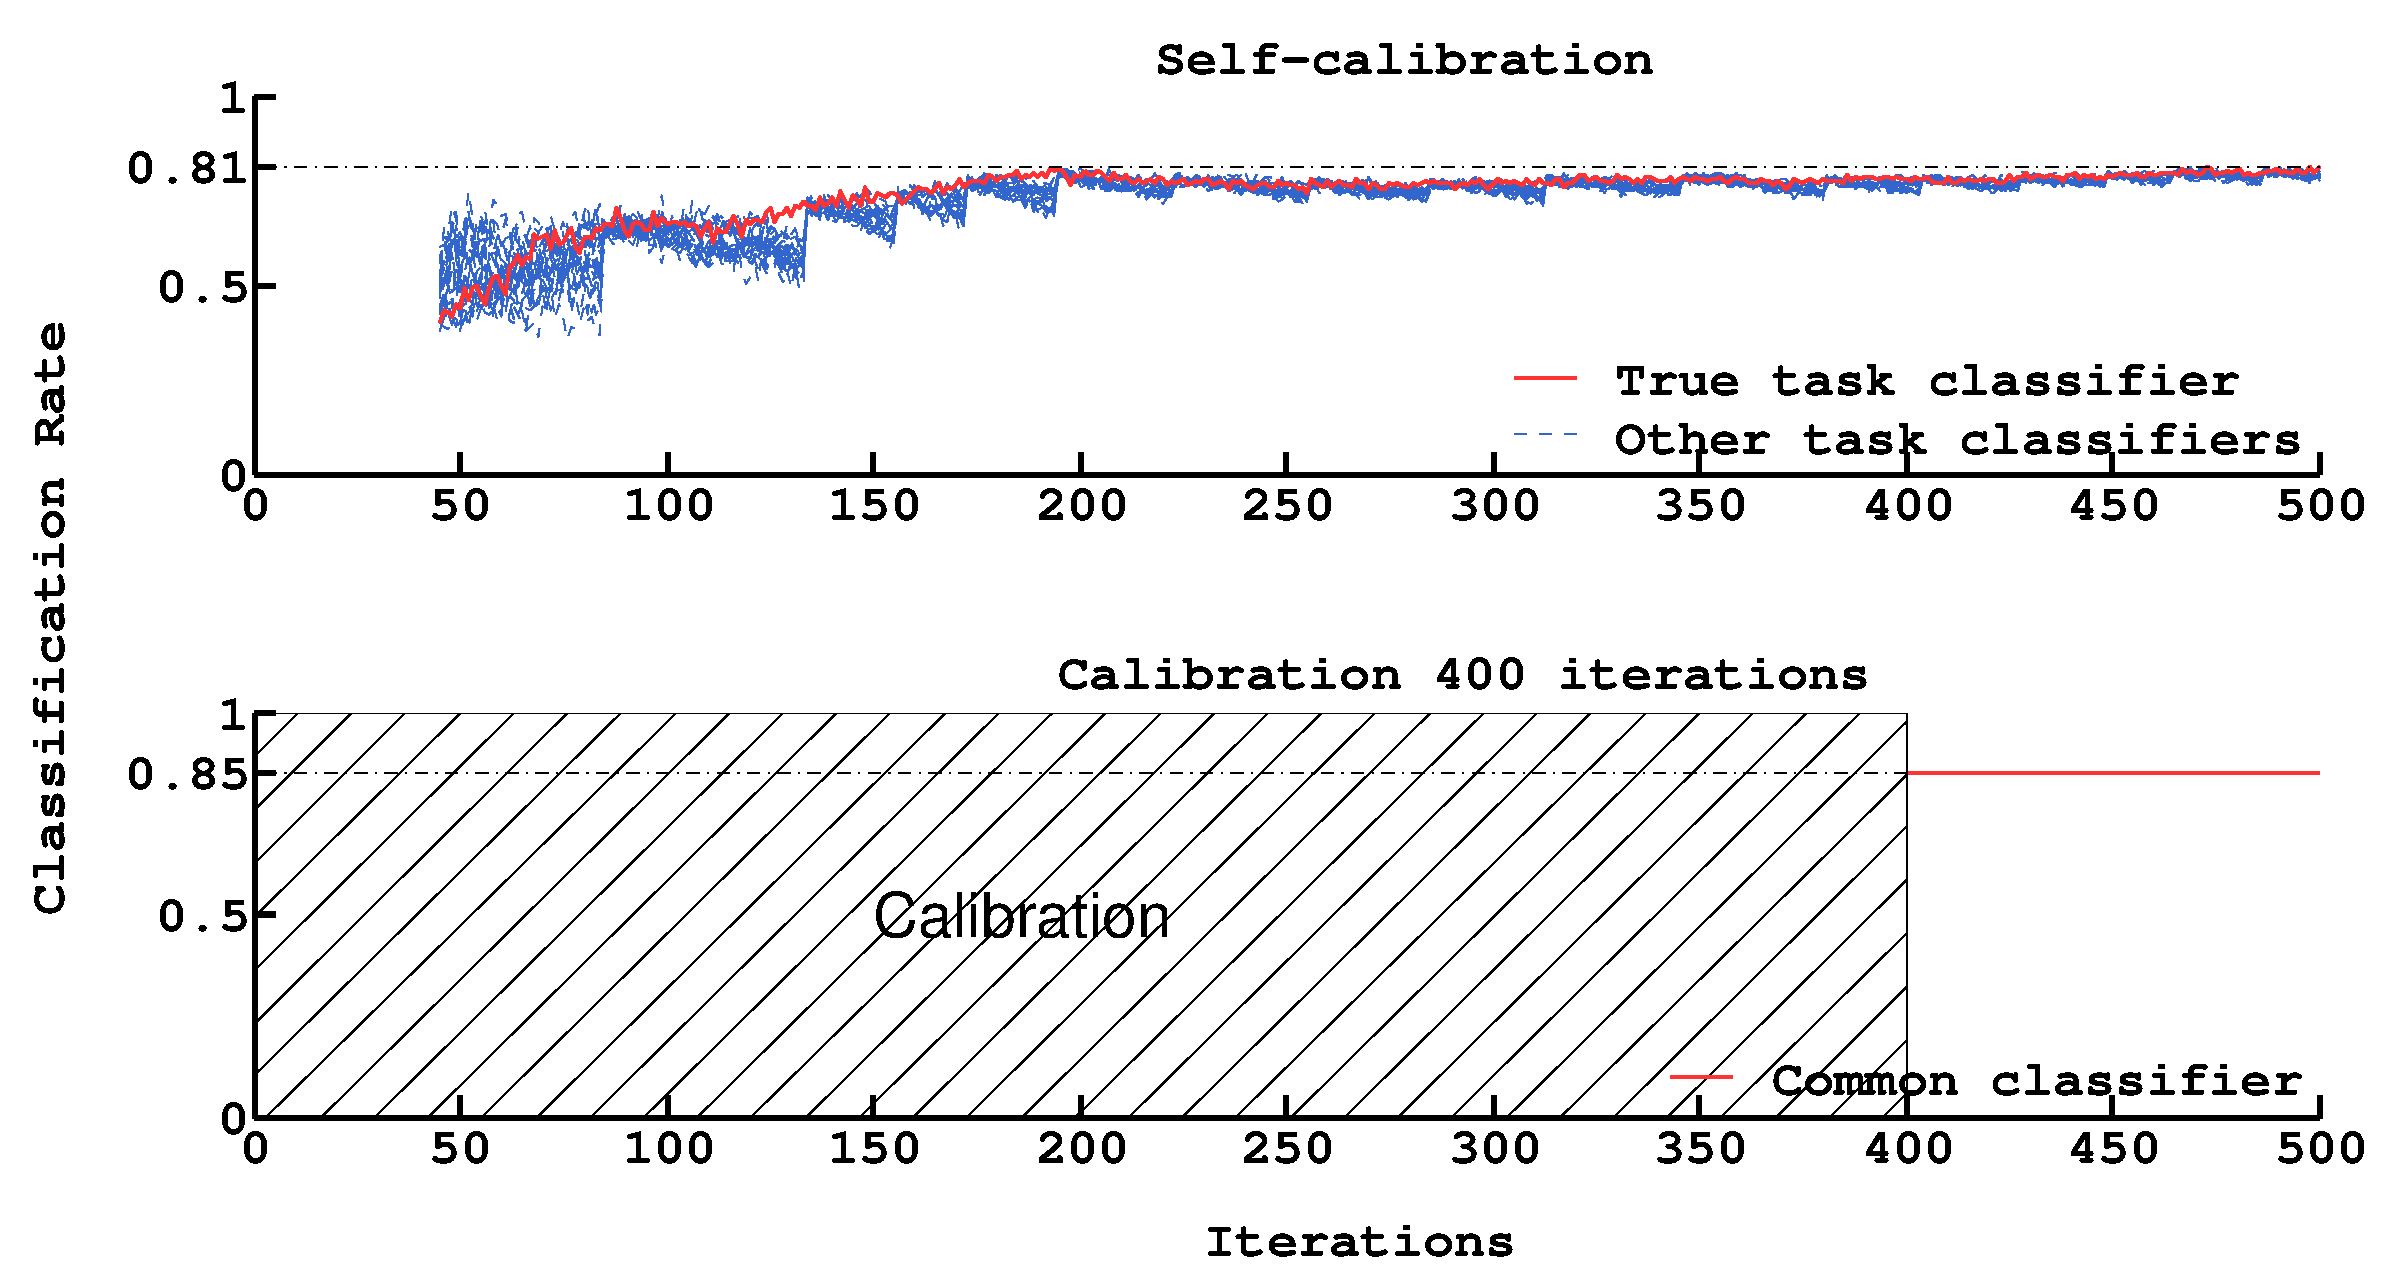
\includegraphics[width=0.8\columnwidth]{images/plot_evo_classification_rate}
\end{center}

We present results from a goal reaching task using real EEG data. We introduce a measure of uncertainty on the task and on the EEG signals interpretation to act as an exploratory bonus for a planning strategy. This speeds up learning by guiding the system to regions that better disambiguate among task hypotheses. 

\vspace{0.5cm}

\begin{center}
\begin{minipage}{.46\columnwidth}
	\begin{center}
		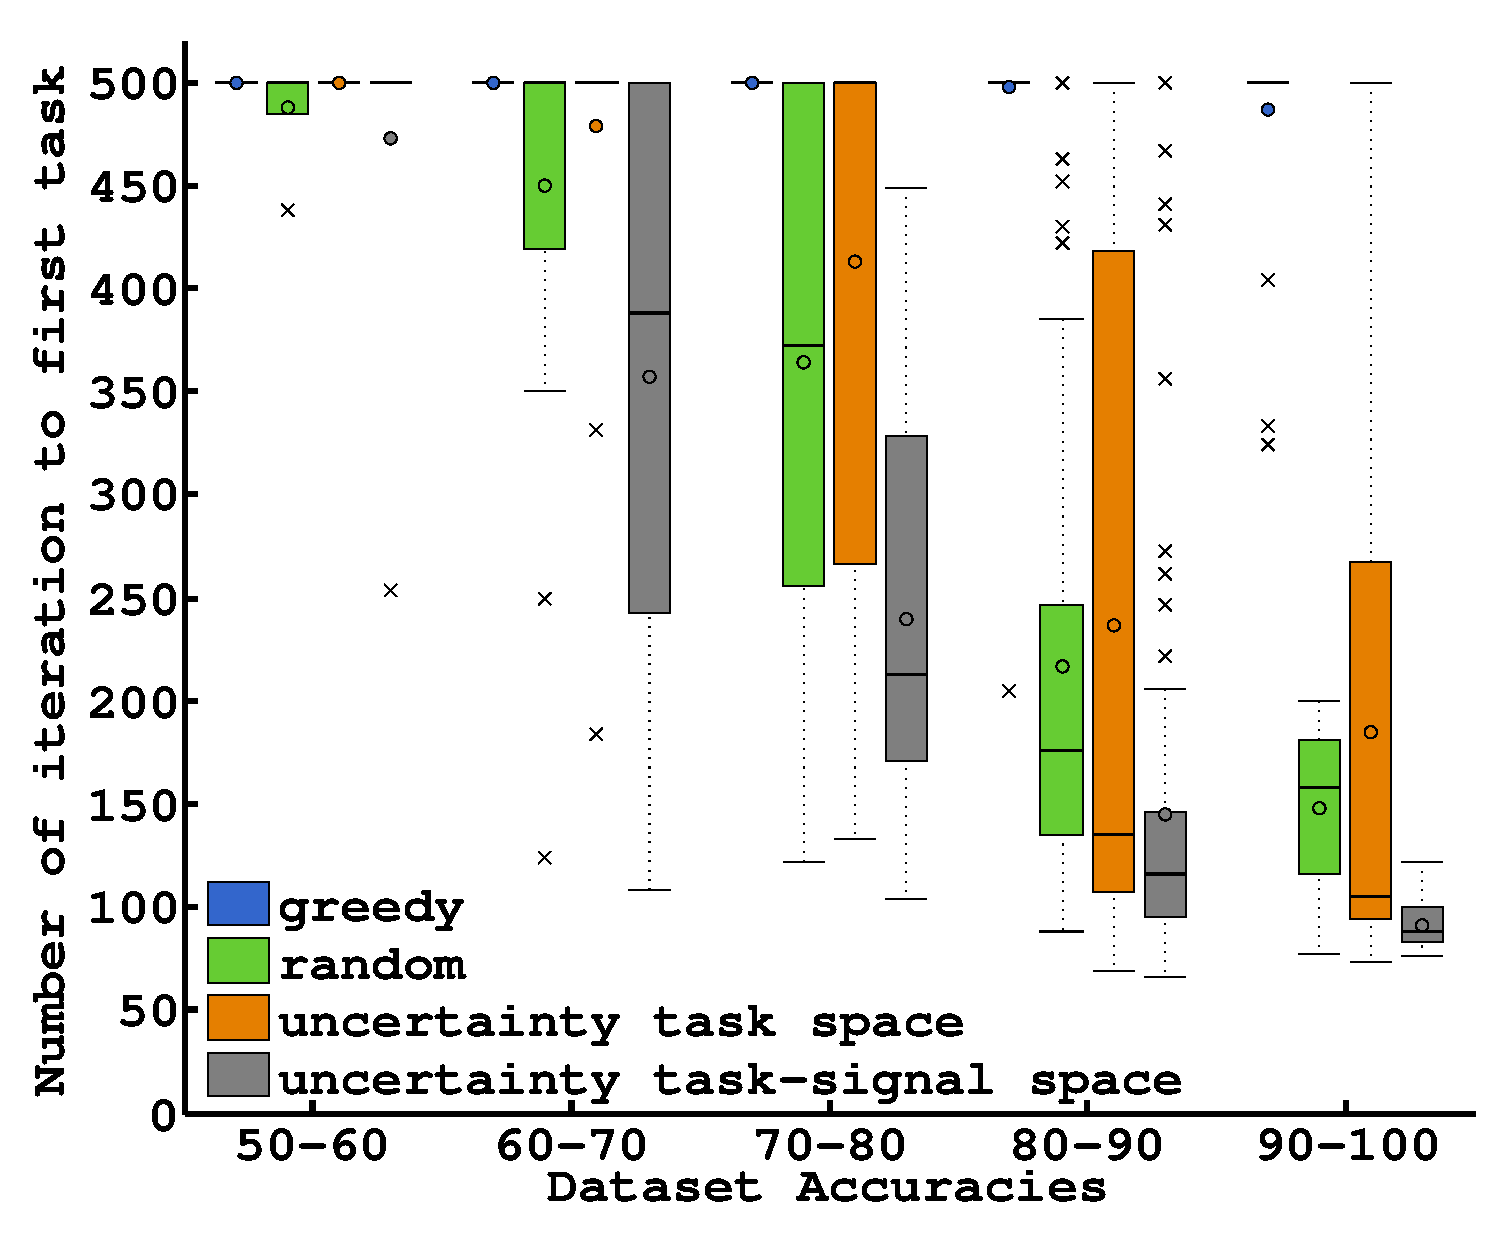
\includegraphics[width=\columnwidth]{images/plot_EEG_planning}
	\end{center}
\end{minipage}
\begin{minipage}{.02\columnwidth}
	\begin{center}

	\end{center}
\end{minipage}
\begin{minipage}{.442\columnwidth}
	\begin{center}
		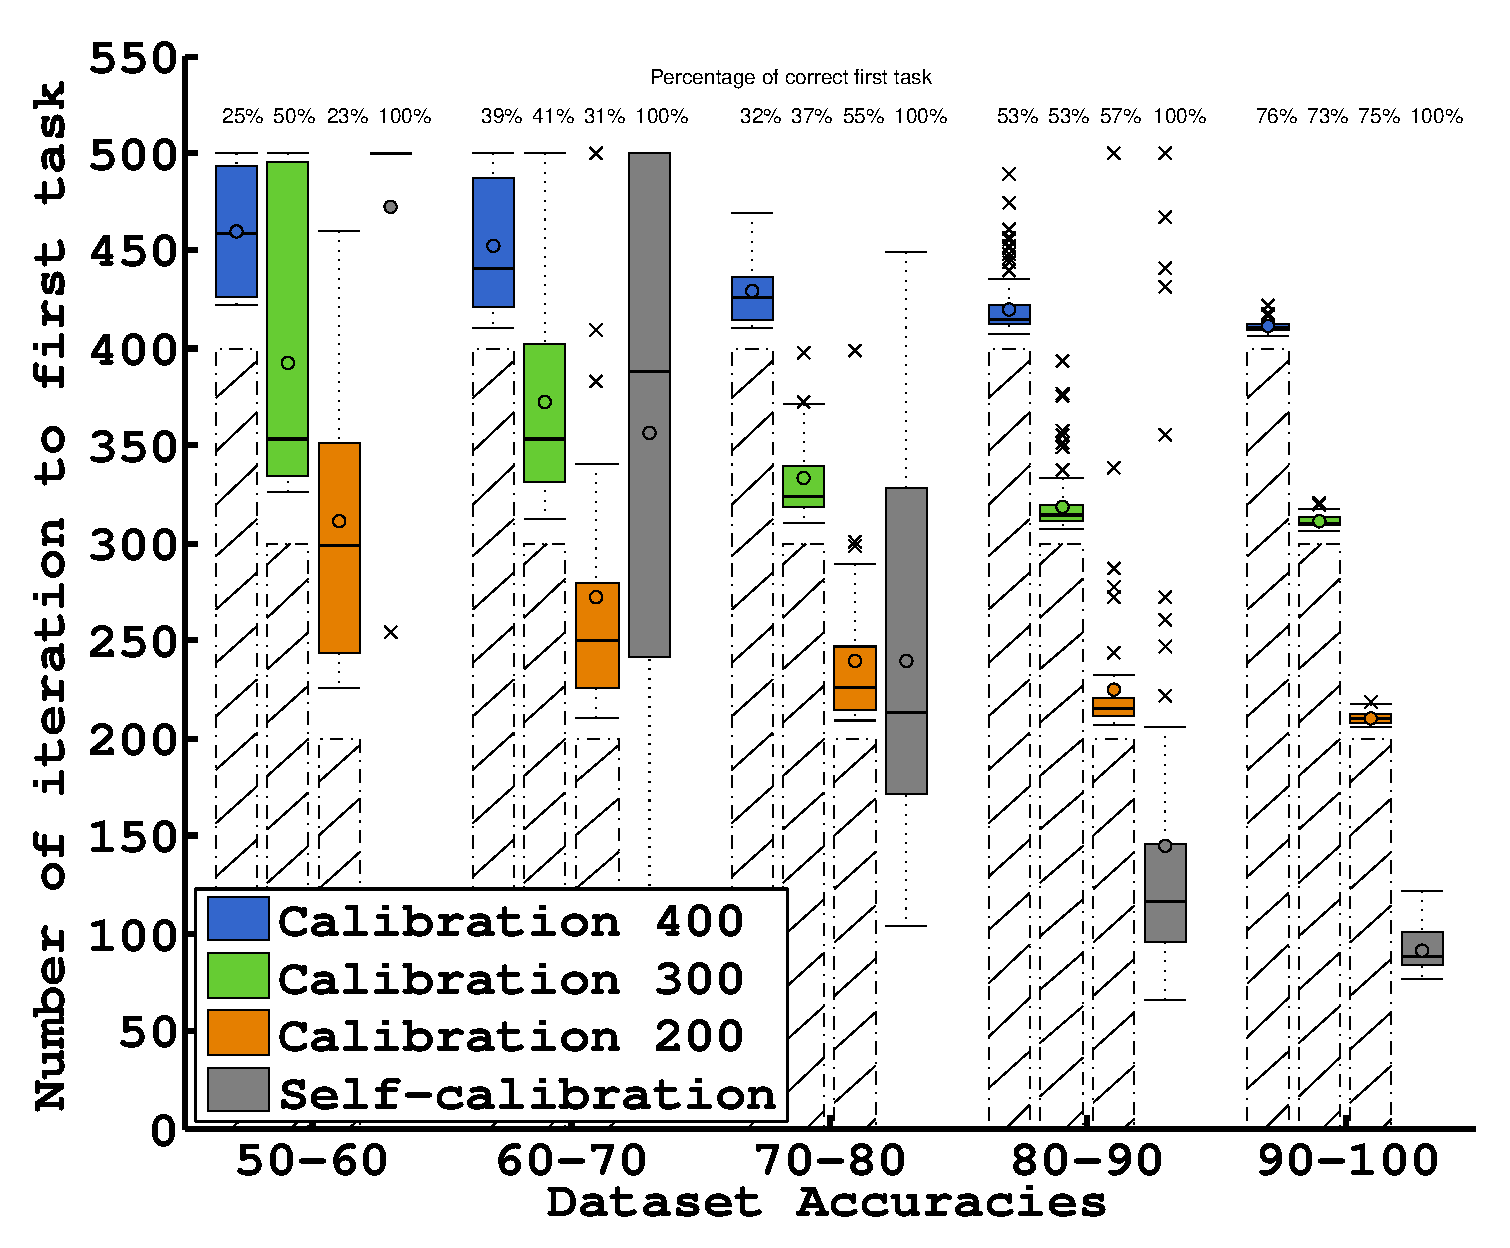
\includegraphics[width=\columnwidth]{images/plot_EEG_calib_firstconf}
	\end{center}
\end{minipage}
\end{center}

We show that we can identify an average of 15 tasks in 500 iterations for EEG dataset of reasonably good quality. We compare our results with a method relying on a calibration procedure, and show that our method allow to learn more tasks in a more reliable way.

\vspace{0.5cm}

\begin{center}
\begin{minipage}{.46\columnwidth}
	\begin{center}
		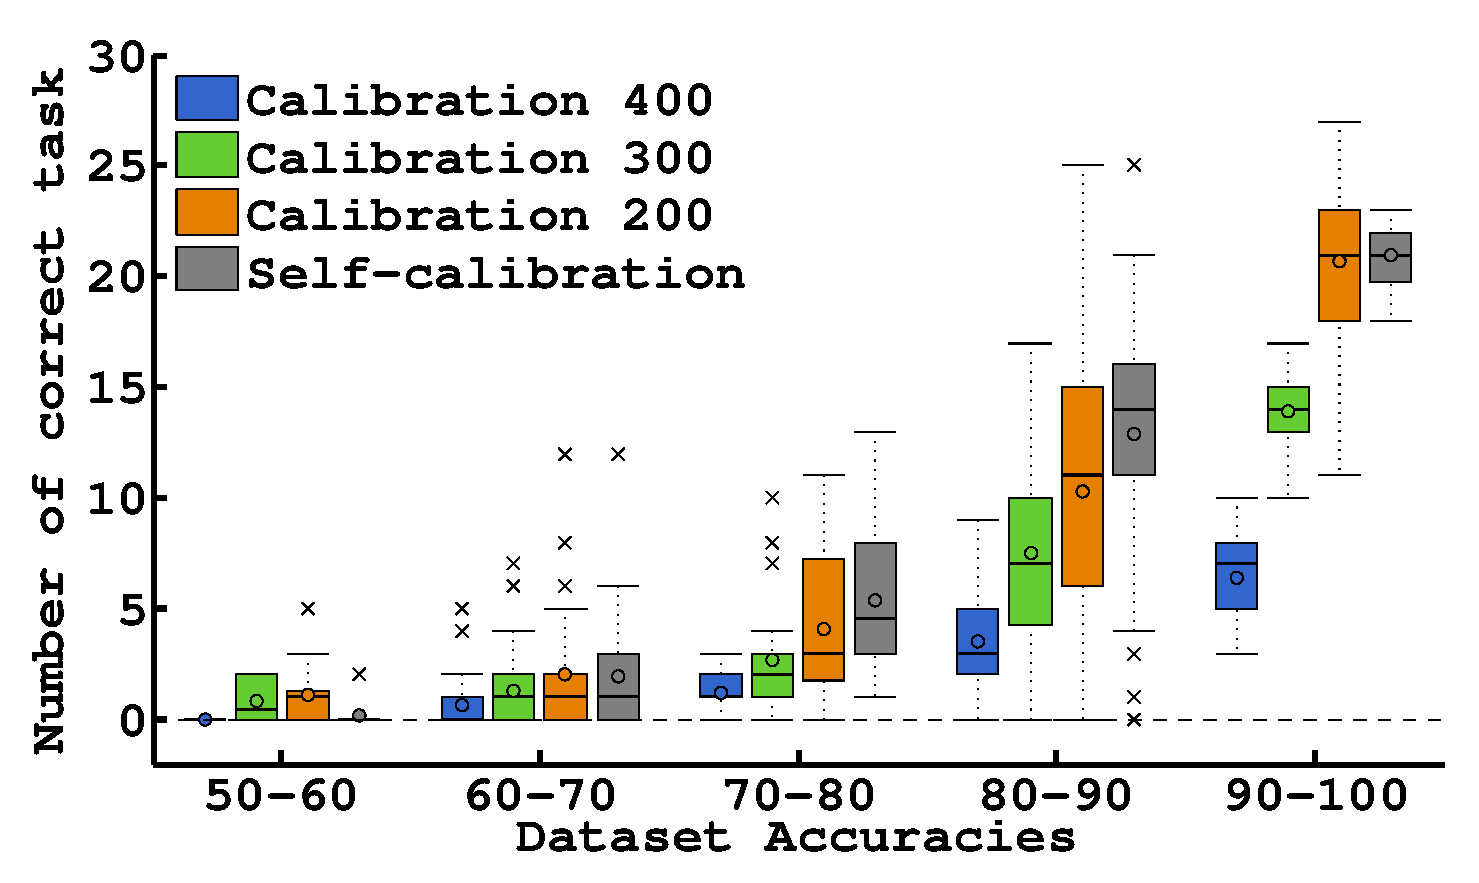
\includegraphics[width=\columnwidth]{images/plot_EEG_calib_nCorrect}	
	\end{center}
\end{minipage}
\begin{minipage}{.02\columnwidth}
	\begin{center}

	\end{center}
\end{minipage}
\begin{minipage}{.442\columnwidth}
	\begin{center}
		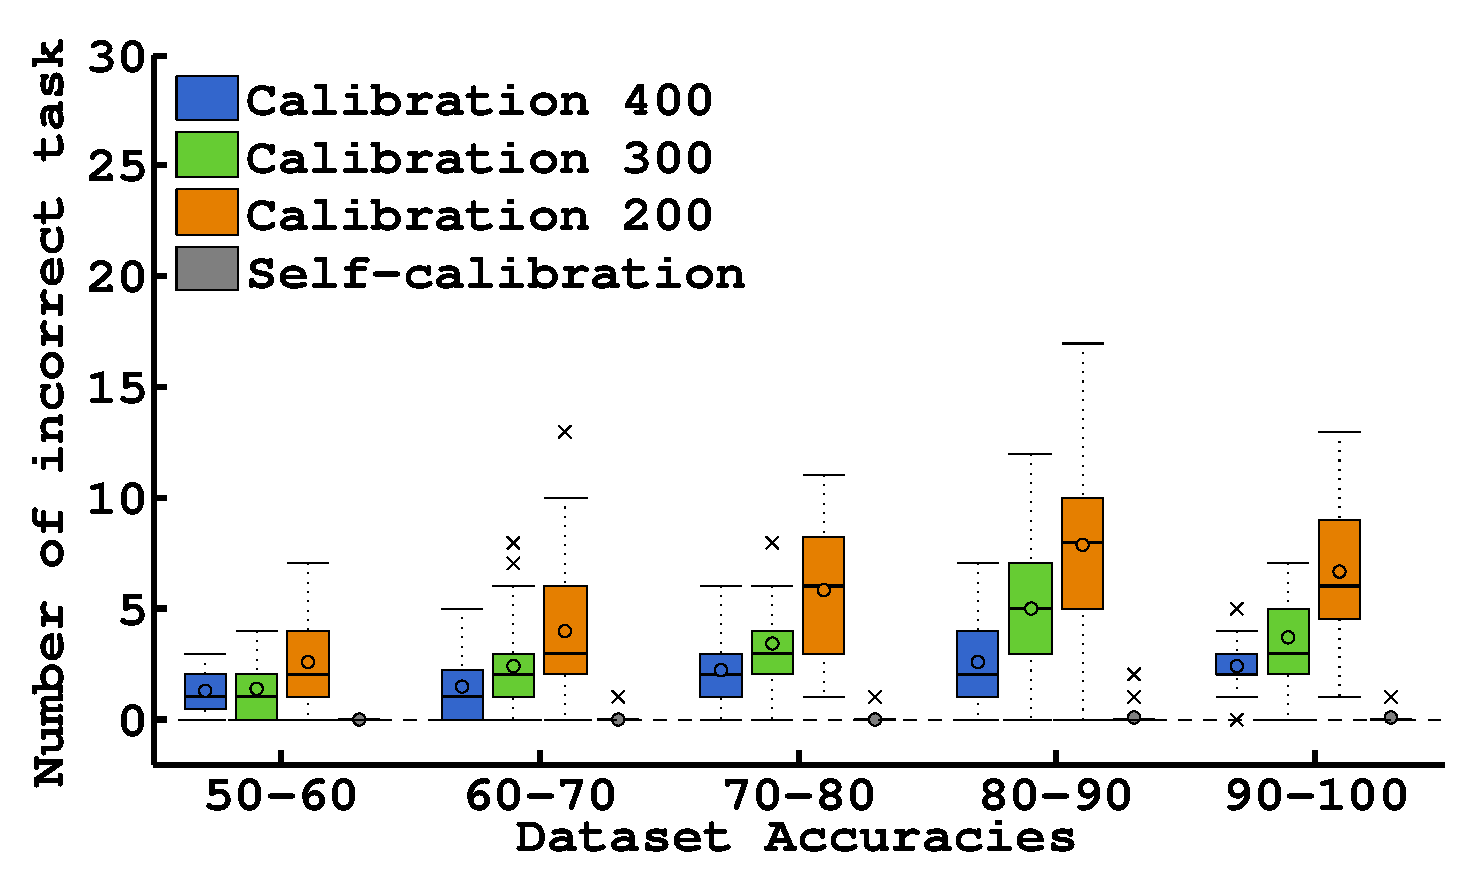
\includegraphics[width=\columnwidth]{images/plot_EEG_calib_nWrong}	
	\end{center}
\end{minipage}
\end{center}

}

\block{References}
{
	% \vspace{-10pt}
	\nocite{*}
	\bibliographystyle{abbrv}
	\renewcommand{\section}[2]{}% Hack to remove bibliography title
	\bibliography{ref}
	\vspace{-10pt}
}

\end{multicols}
\vfill
\end{document}
